% !Mode:: "TeX:UTF-8"
%% 请使用 XeLaTeX 编译本文.
 \documentclass[forprint]{report}
%---------------------这里添加所需的package--------------------------------
\usepackage{url}
\usepackage{amsmath}

%--------------------------------------------------------------------------
\makeatletter
\def\BState{\State\hskip-\ALG@thistlm}
\makeatother
\begin{document}
%-----------------------------------------------------------------------------

\title{过拟合} % 报告主题
\author{曾文正} % 学生姓名
\Csupervisor{袁烨} % 指导教师姓名
\CstudentNum{U201715853} % 学号
\Cmajor{自动化校交1701} % 专业名称
\Cschoolname{人工智能与自动化学院} % 学院名
\date{2020年6月20日} % 日期

%-----------------------------------------------------------------------------

\pdfbookmark[0]{封面}{title}         % 封面页加到 pdf 书签
\maketitle
\frontmatter
\pagenumbering{Roman}              % 正文之前的页码用大写罗马字母编号.正文之前的页码隐藏,无需显示
%-----------------------------------------------------------------------------
%==========================把目录加入到书签==============================%%%%%%

\tableofcontents
\thispagestyle{empty}				%不显示罗马数字
\addtocontents{toc}{\protect\thispagestyle{empty}}


\mainmatter %% 以下是正文
%%%%%%%%%%%%%%%%%%%%%%%%%%%--------main matter-------%%%%%%%%%%%%%%%%%%%%%%%%%%%%%%%%%%%%
\pagestyle{plain}%plain
%\cfoot{\thepage{\zihao{5}\bf\usefonttimes}}
%\renewcommand{\baselinestretch}{1.6}
%\setlength{\baselineskip}{23pt}
\baselineskip=23pt  % 正文行距为 23 磅

%此处书写正文-------------------------------------------------------------------------------------
\chapter{摘要}
本文首先直观地描述了欠拟合与过拟合,然后用两种角度在理论上解释了模型复杂度与欠拟合、过拟合的关系:第一种角度是从方差、偏差分解的角度,方差体现泛化性能,偏差体现拟合好坏。第二种角度是VC维,思路是希望从理论上推导出真实表现与训练时表现的差距的量化关系。从霍夫丁不等式一步步推导,最后引出VC的概念来量化真实表现与训练表现间的差距,从而建立了模型复杂度、样本个数与欠拟合、过拟合间的关系。之后,我介绍了防止过拟合的方法,先是较为详尽地介绍了正则化:从直观的出发点解释了正则化的意义,并从贝叶斯角度推导出Lasso回归和岭回归的损失函数,并从先验概率和梯度两个角度解释了L1、L2正则化的区别,然后介绍了综合这两种正则化优点的弹性网络。接着介绍了数据增强、提前停止训练等方法,交叉验证是一种很好地评估模型性能的方法,用于评估模型性能,也可用来选择模型。同时,我也介绍了防止欠拟合的方法,相对来说防止欠拟合要比防止过拟合简单得多。最后通过自己编程实现了线性回归和岭回归,发现岭回归确实起到了提高模型泛化性能的作用,并且不同的系数会有不同的效果。实验的结果与理论相符。
\chapter{欠拟合与过拟合}
\section{欠拟合、过拟合的直观描述}
\begin{figure}[ht]
	\centering
	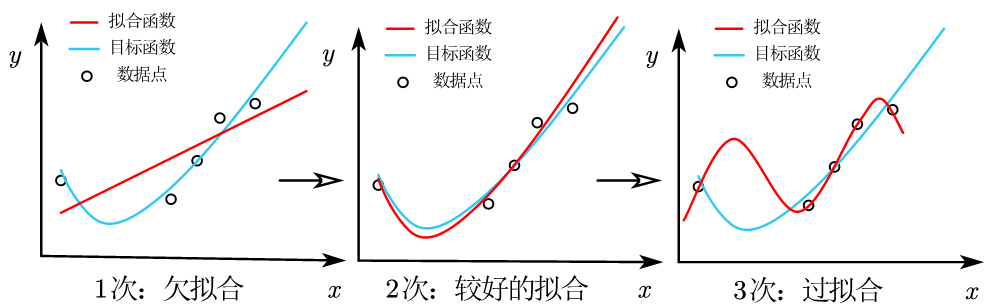
\includegraphics[width=\textwidth]{overfit.png}
	\caption{过拟合直观描述}
	\label{fig:1}
\end{figure}
假设给定真实的目标函数为f(x),每个数据点y=f(x)+噪声。用它生成了5个点作为训练数据集。如果我们使用1次多项式进行拟合,发现拟合效果并不好,直观的感受是由于模型过于简单,使得该模型不能很好地学习到训练集的特征,这就是欠拟合现象。如果我们使用2次多项式进行拟合,发现拟合的效果还可以,接近目标函数。如果我们使用4次多项式进行拟合,可以使拟合曲线经过这5个点,也就是在训练集上的误差为0。但实际上可以看出我们拟合出的5次多项式和真实的目标函数f差很远。因为训练数据集是有限的,而目标函数我们一般是未知的,在训练集上表现得好不等于在实际中也表现得好,在这个例子中就拟合过度了,导致泛化性能很差,这就是过拟合。一方面是由于有噪声,我们的模型把噪声也拟合进去了;另一方面是由于信息的不充分性,因为这5个点,有无穷多种拟合方式都能保证0误差,但与目标函数接近的远没有那么多。因此如果模型过于复杂可以让训练误差很小,但可能会偏离真实目标函数而造成过拟合。
\section{偏差与方差角度解释欠、过拟合}
\subsection{偏差方差分解的推导}
在机器学习中,我们用训练数据集去训练一个模型,通常的做法是定义一个误差函数,通过将这个误差最小化,来提高模型的性能。然而学习一个模型的目的是为了解决训练数据集这个领域中的一般化问题,单纯地将训练数据集的损失最小化,并不能保证在解决更一般的问题时模型仍然是最优,甚至不能保证模型是可用的。这个训练数据集的损失与一般化的数据集的损失之间的差异就叫做泛化误差。而泛化误差可以分解为偏差、方差和噪声。

如果能够获得所有可能的数据集合,并在这个数据集合上将损失最小化,那么学习得到的模型就可以称之为“真实模型”。当然,在现实生活中我们不可能获取并训练所有可能的数据,所以“真实模型”肯定存在,但是无法获得。我们的最终目的是学习一个模型使其更加接近这个真实模型。

偏差和方差分别从两个方面来描述我们学习到的模型与真实模型之间的差距。下面对偏差、方差和噪声进行定义。
\paragraph*{符号说明:}
$E_D$指在数据集D上取期望,$g\left(x\right)$指通过数据集D训练得到的模型,$y$指真实的标签,$y_D$指数据集的标签(即可能在真实标签的基础上带有噪声)。

\noindent
偏差:
$$
bias^2\left( x \right) =\left( E_D\left[ g\left( x \right) \right] -y \right) ^2
$$
偏差度量的是训练得到的模型的期望预测与真实结果的偏离程度,刻画的是拟合能力。

\noindent
方差:
$$
var\left( x \right) =E_D\left[ \left( g\left( x \right) -E_D\left[ g\left( x \right) \right] \right) ^2 \right] 
$$
方差度量的是数据集变动带来的训练模型性能的波动,刻画的是泛化能力。

\noindent
噪声:
$$
\varepsilon =E_D\left[ \left( y_D-y \right) ^2 \right] 
$$
噪声是获取的数据和理想数据间的差异,反应了学习问题本身的难度下限。

\noindent
由此我们可以推导,将泛化误差分解为偏差+方差+噪声:
\begin{small}
	$$
	\begin{aligned}
	err&=E_D\left[ \left( g\left( x \right) -y_D \right) ^2 \right] 
	\\
	&=E_D\left[ \left( g\left( x \right) -E_D\left[ g\left( x \right) \right] +E_D\left[ g\left( x \right) \right] -y_D \right) ^2 \right] 
	\\
	&=E_D\left[ \left( g\left( x \right) -E_D\left[ g\left( x \right) \right] \right) ^2 \right] +E_D\left[ \left( E_D\left[ g\left( x \right) \right] -y_D \right) ^2 \right] +2E_D\left[ \left( g\left( x \right) -E_D\left[ g\left( x \right) \right] \right) \left( E_D\left[ g\left( x \right) \right] -y_D \right) \right] 
	\\
	&=E_D\left[ \left( g\left( x \right) -E_D\left[ g\left( x \right) \right] \right) ^2 \right] +E_D\left[ \left( E_D\left[ g\left( x \right) \right] -y_D \right) ^2 \right] 
	\\
	&=E_D\left[ \left( g\left( x \right) -E_D\left[ g\left( x \right) \right] \right) ^2 \right] +E_D\left[ \left( E_D\left[ g\left( x \right) \right] -y+y-y_D \right) ^2 \right] 
	\\
	&=E_D\left[ \left( g\left( x \right) -E_D\left[ g\left( x \right) \right] \right) ^2 \right] +E_D\left[ \left( E_D\left[ g\left( x \right) \right] -y \right) ^2 \right] +E_D\left[ \left( y-y_D \right) ^2 \right] +2E_D\left[ \left( E_D\left[ g\left( x \right) \right] -y \right) \left( y-y_D \right) \right] 
	\\
	&=\left( E_D\left[ g\left( x \right) \right] -y \right) ^2+E_D\left[ \left( g\left( x \right) -E_D\left[ g\left( x \right) \right] \right) ^2 \right] +E_D\left[ \left( y_D-y \right) ^2 \right] 
	\\
	&=bias^2\left( x \right) +var\left( x \right) +\varepsilon 
	\end{aligned}
	$$
\end{small}

\subsection{偏差、方差、模型复杂度与欠拟合、过拟合间的关系}
\begin{figure}[ht]
	\centering
	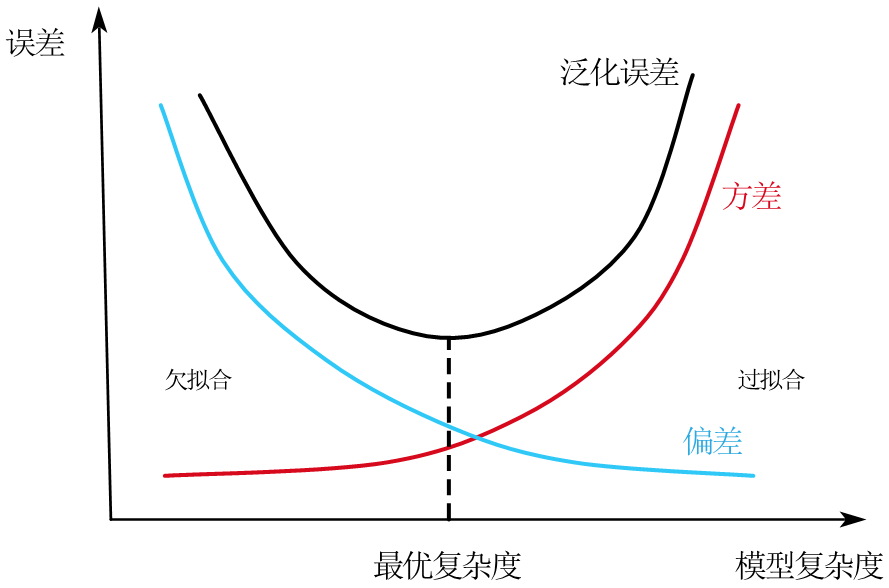
\includegraphics[width=\textwidth]{bias_var.png}
	\caption{偏差方差与模型复杂度间的关系}
	\label{fig:1}
\end{figure}
模型复杂度过低,则偏差大,方差小,泛化误差大;模型复杂度过大,则偏差小,方差大,泛化误差大;只有在模型复杂度适中时泛化误差最小。在模型简单时,发生欠拟合,即模型不能适配样本,有一个很大的偏差。在模型过于复杂时,发生过拟合,即模型将训练集数据拟合地很好,但拟合的过好导致泛化性能差,也就是有一个很大的方差。
\section{VC维角度解释欠、过拟合}
第二种训练模型的思路是,先保证训练误差接近0,然后再考虑让真实误差接近训练误差,那么这样真实误差也可以接近0了。
\subsection{铺垫——有限个假设的情况}
机器学习问题可以理解为通过训练集数据,在假设集H中,通过学习算法A找到H中最好的一个假设h作为$g$,使得$g\approx f$(f为未知的目标函数)我们用训练误差代表训练集拟合情况,用泛化误差代表真实的性能好坏。假设研究二分类问题,且训练集与真实的样本服从同一分布P,对于假设h,定义训练误差为:$$
E_{in}\left( h \right) =\frac{1}{N}\sum_{i=1}^N{\left\{ h\left( x_i \right) \ne f\left( x_i \right) \right\}}
$$泛化误差为:
$$
E_{out}\left( h \right) =E_{x \sim p}\left\{ h\left( x \right) \ne f\left( x \right) \right\} 
$$
其中$\left\{  \right\} $是bool函数,返回其内部的真(1)假(0)。

\noindent
引理1:霍夫丁不等式:
$$
P\left( \left| E_{in}\left( h \right) -E_{out}\left( h \right) \right|>\varepsilon \right) \leqslant 2\exp \left( -2\varepsilon ^2N \right) 
$$其中N为数据集内样本的个数。
从这个式子可以看出对于给定的某个固定的 $h$,假如训练集规模$N$很大的时候,训练误差很接近泛化误差的概率是很高的。然而不仅需要对于针对某一个特定的 $h$ 的时候能保证 $E_{out}\left( h \right)$ 接近 $E_{in}\left( h \right)$ 且接近的概率很高。我们还要证明同时针对所有的$h\in H$这个结论都成立。通过联合联合约束就可以得到下面的关系:
$$
\begin{aligned}
P\left( \exists h\in H.\left| E_{in}\left( h_i \right) -E_{out}\left( h_i \right) \right|>\varepsilon \right)&\leqslant \sum_{i=1}^m{P\left( \left| E_{in}\left( h_i \right) -E_{out}\left( h_i \right) \right|>\varepsilon \right)}
\\
&=2m\exp \left( -2\varepsilon ^2N \right) 
\end{aligned}
$$
其中m为假设的个数。通过这个约束可以知道,至少有 $
1-2m\exp \left( -2\varepsilon ^2N \right) 
$的概率,我们能确保对于所有的$h\in H$,$E_{out}$ 在 $E_{in}$ 附近 $\varepsilon $ 范围内。也就是说我们可以量化训练误差与实际泛化误差的接近程度及其概率。如果我们可以训练得到一个h使得$E_{in}$约等于0,那么在样本数据极大的时候,我们就可以通过控制上述公式中的参数做到$E_{out}$约等于$E_{in}$。
\subsection{无限个假设的情况——引出VC维}
注意到一般情况下研究的是有无限个假设的情况(比如线性回归,w在R内取值,是无限多个的),如果把刚刚得到的结论直接用于无限个假设的情况显然是不行的,因为等式右边无限项的和会超过1,而概率是不能大于1的。原因是因为上面推导的时候利用了联合概率约束,这是个十分宽松的约束,因为在假设集中有很多假设得到的结果是极为相似的。因此可以考虑把无限个假设划分为多个有限的类,在每一类内的假设表现相同。

我们来考虑二分类问题。假设有N个数据点,那么它们的分类组合情况最多有$2^N$种,因此这时我们就可以把趋近于无穷的M缩小为$2^N$。但这还是一个比较宽松的上界。

实际上,我们的假设模型可能不能把所有的这$2^N$种情况都展现出来,也就是说我们的假设模型可能无法区分其中的多种情况。这实际上体现的是这个模型的复杂程度,模型越复杂则越能表达出更多种分类情况,模型越简单则只能表达出较少的分类情况,其他许多情况无法表达。同时,这也进一步把我们的上界缩小了。也就是能够通过理论更准确得由$E_{in}$控制$E_{out}$的界限了。

这里就可以引入VC维的概念了:给定一个假设类H,VC维这个值是能被H打散的最大的数据集规模。打散指的就是H能够表达出所有$2^N$种情况。VC维体现了这个假设的复杂程度。
通过数学推导可以得到一个定理$$
P\left( \left| E_{in}-E_{out} \right|>\varepsilon \right) \leqslant 4\left( 2N \right) ^{d_{vc}}\exp \left( -\frac{1}{8}\epsilon ^2N \right) 
$$进而可以得到:\\
\noindent
设$\delta =4\left( 2N \right) ^{d_{vc}}\exp \left( -\frac{1}{8}\varepsilon ^2N \right)$,则有
$$
\begin{aligned}
\frac{\delta}{4\left( 2N \right) ^{d_{vc}}}&=\exp \left( -\frac{1}{8}\varepsilon ^2N \right) 
\\
\ln \left( \frac{4\left( 2N \right) ^{d_{vc}}}{\delta} \right) &=\frac{1}{8}\varepsilon ^2N
\\
\ \varepsilon &=\sqrt{\frac{8}{N}\ln \left( \frac{4\left( 2N \right) ^{d_{vc}}}{\delta} \right)}
\end{aligned}
$$
这说明:$$
\text{有}1-\delta \text{的概率使:}E_{out}\leqslant E_{in}+\sqrt{\frac{8}{N}\ln \left( \frac{4\left( 2N \right) ^{d_{vc}}}{\delta} \right)}
$$
%\clearpage
\begin{figure}[ht]
	\centering
	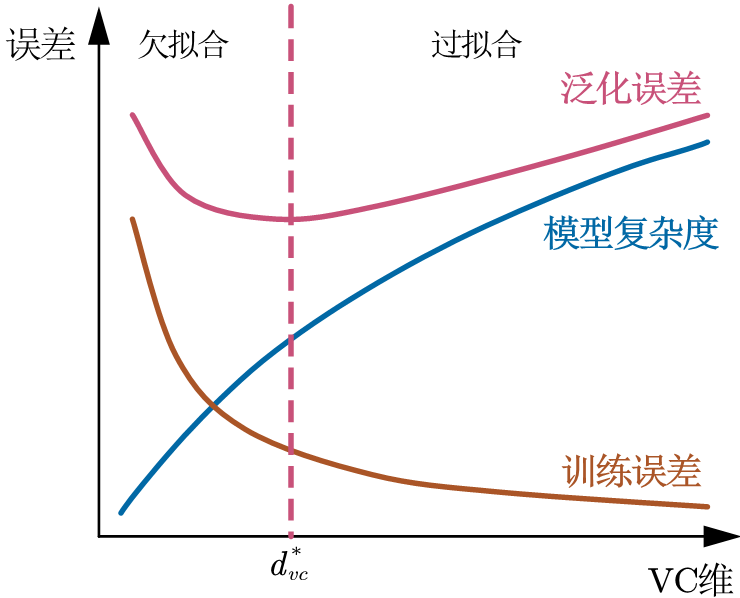
\includegraphics[width=\textwidth]{dvc.png}
	\caption{VC维与模型复杂度、欠拟合、过拟合间的关系}
	\label{fig:1}
\end{figure}

将这个公式具体化为图像,我们可以得到VC维与模型复杂度、训练误差、泛化误差之间的关系。如图2.3,可以看出VC基本与模型复杂度成线性关系,也就是VC维可以代表模型复杂度。随着模型复杂度的增大,训练误差一直减少,泛化误差先减小后增大。

VC维很小时,训练误差和泛化误差都大,这时对应欠拟合。随着VC维的增大,训练误差减小,泛化误差先减小后增大,泛化误差的极值点对应的就是最优的VC维,随后,若VC维继续增大,则训练误差继续减小,但泛化误差开始增大,这时对应过拟合。
\chapter{防止过拟合的方法}
\section{正则化——避免过拟合的方法}
\subsection{直观理解正则化的出发点}
直观上理解,模型参数的个数越多,模型的复杂度越高。由前面的分析可以知道,模型复杂可能带来过拟合的现象。因此我们可以通过减少模型参数的方法来减小模型的复杂度,这可以理解为让其中的一些参数等于0。如果说把条件再放宽松一点,那我们希望让各参数都尽量接近于0,这也训练得到的曲线会更加平滑。这就是正则化想要做的。
\subsection{$L_1,L_2$正则化概念综述}
$L_1$正则化(Lasso回归)、$L_2$正则化(岭回归)是比较常用的正则化方法,是对线性回归的改进,在其损失函数基础上加入一个正则项来让权值尽量接近0,防止过拟合。

\noindent
Lasso回归定义为:
$$
\min_w \left[ \sum_{i=1}^N{\left( y_i-w^Tx_i \right) ^2+\lambda \lVert w \rVert _1} \right] 
$$
岭回归定义为:
$$
\min_w \left[ \sum_{i=1}^N{\left( y_i-w^Tx_i \right) ^2+\lambda \lVert w \rVert _{2}^{2}} \right] 
$$
\subsection{从贝叶斯角度推导$L_1,L_2$正则化}
\subsubsection{Lasso回归推导}
对于线性回归,我们假设真实值存在一个分布为$N\left( 0,\sigma ^2 \right)$的噪声$\varepsilon$ ,即对于每一个样本有:
$$
y_i=w^Tx_i+\varepsilon 
$$
$$
p\left( y_i|x_i,w \right) \sim N\left( w^Tx_i,\sigma ^2 \right) 
$$
$$
p\left( y_i|w \right) =\frac{1}{\sqrt{2\pi}\sigma}\exp \left( -\frac{\left( y_i-w^Tx_i \right) ^2}{2\sigma ^2} \right) 
$$
从之前的直观理解正则化出发点中的分析可知,我们希望得到的w的各分量都接近于0,那么我们就假设w服从均值为0的拉普拉斯分布,即
$$
p\left( w \right) =\frac{1}{2\sigma _0}e^{-\frac{\lVert w \rVert _1}{\sigma _0}}
利用最大后验估计可得:
$$
$$
\begin{aligned}
\widehat{w}&=\underset{w}{arg\max}p\left( w|Y \right) 
\\
&=\underset{w}{arg\max}\left[ p\left( w \right) p\left( Y|w \right) \right] 
\\
&=\underset{w}{arg\max}\left[ p\left( w \right) \prod_{i=1}^N{p\left( y_i|w \right)} \right] 
\\
&=\underset{w}{arg\max}\ln \left[ p\left( w \right) \prod_{i=1}^N{p\left( y_i|w \right)} \right] 
\\
&=\underset{w}{arg\max}\left[ \ln p\left( w \right) +\sum_{i=1}^N{\ln p\left( y_i|w \right)} \right] 
\\
&=\underset{w}{arg\max}\left[ \ln \left( \frac{1}{2\sigma _0}e^{-\frac{\lVert w \rVert _1}{\sigma _0}} \right) +\sum_{i=1}^N{\ln \left( \frac{1}{\sqrt{2\pi}\sigma}e^{-\frac{\left( y_i-w^Tx_i \right) ^2}{2\sigma ^2}} \right)} \right] 
\\
&=\underset{w}{arg\max}\left[ \ln \frac{1}{2\sigma _0}+\ln \left( e^{-\frac{\lVert w \rVert _1}{\sigma _0}} \right) +\sum_{i=1}^N{\ln \frac{1}{\sqrt{2\pi}\sigma}}+\sum_{i=1}^N{\ln \left( e^{-\frac{\left( y_i-w^Tx_i \right) ^2}{2\sigma ^2}} \right)} \right] 
\\
&=\underset{w}{arg\min}\left[ \frac{\lVert w \rVert _1}{\sigma _0}+\sum_{i=1}^N{\frac{\left( y_i-w^Tx_i \right) ^2}{2\sigma ^2}} \right] 
\\
&=\underset{w}{arg\min}\left[ \sum_{i=1}^N{\left( y_i-w^Tx_i \right) ^2+\frac{2\sigma ^2}{\sigma _{0}^{2}}\lVert w \rVert _1} \right] 
\\
&=\underset{w}{arg\min}\left( \lVert Y-Xw \rVert _{2}^{2}+\lambda \lVert w \rVert _1 \right) 
\end{aligned}
$$
\subsubsection{岭回归推导}
和Lasso回归类型,只不过区别在于岭回归的先验概率是w服从均值为0的高斯分布,即
$$
p\left( w \right) =\frac{1}{\sqrt{2\pi}\sigma _{0}^{2}}e^{-\frac{\lVert w \rVert _{2}^{2}}{2\sigma _{0}^{2}}}
$$
利用最大后验估计可得:
$$
\begin{aligned}
\hat{w}
%\hat{w}\begin{matrix}{l}
&=\underset{w}{arg\max}p\left( w|Y \right)\\
&=\underset{w}{arg\max}\left[ p\left( w \right) p\left( Y|w \right) \right]\\
&=\underset{w}{arg\max}\left[ p\left( w \right) \prod_{i=1}^N{p\left( y_i|w \right)} \right]\\
&=\underset{w}{arg\max}\ln \left[ p\left( w \right) \prod_{i=1}^N{p\left( y_i|w \right)} \right]\\
&=\underset{w}{arg\max}\left[ \ln p\left( w \right) +\sum_{i=1}^N{\ln p\left( y_i|w \right)} \right]\\
&=\underset{w}{arg\max}\left[ \ln \left( \frac{1}{\sqrt{2\pi}\sigma _0}e^{-\frac{\lVert w \rVert _{2}^{2}}{2\sigma _{0}^{2}}} \right) +\sum_{i=1}^N{\ln \left( \frac{1}{\sqrt{2\pi}\sigma}e^{-\frac{\left( y_i-w^Tx_i \right) ^2}{2\sigma ^2}} \right)} \right]\\
&=\underset{w}{arg\max}\left[ \ln \frac{1}{\sqrt{2\pi}\sigma _0}+\ln \left( e^{-\frac{\lVert w \rVert _{2}^{2}}{2\sigma _{0}^{2}}} \right) +\sum_{i=1}^N{\ln \frac{1}{\sqrt{2\pi}\sigma}}+\sum_{i=1}^N{\ln \left( e^{-\frac{\left( y_i-w^Tx_i \right) ^2}{2\sigma ^2}} \right)} \right]\\
&=\underset{w}{arg\min}\left[ \frac{\lVert w \rVert _{2}^{2}}{2\sigma _{0}^{2}}+\sum_{i=1}^N{\frac{\left( y_i-w^Tx_i \right) ^2}{2\sigma ^2}} \right]\\
&=\underset{w}{arg\min}\left[ \sum_{i=1}^N{\left( y_i-w^Tx_i \right) ^2+\frac{\sigma ^2}{\sigma _{0}^{2}}\lVert w \rVert _{2}^{2}} \right]\\
&=\underset{w}{arg\min}\left( \lVert Y-Xw \rVert _{2}^{2}+\lambda \lVert w \rVert _{2}^{2} \right)\\
%\end{matrix}
\end{aligned}
$$
并且岭回归还有一个优点就是可以利用矩阵运算直接求得最优解。
$$
\begin{aligned}
h\left( x \right) 
&=\lVert Y-Xw \rVert _{2}^{2}+\lambda \lVert w \rVert _{2}^{2}\\
&=\left( Y-Xw \right) ^T\left( Y-Xw \right) +\lambda w^Tw\\
&=\left[ Y^T-\left( Xw \right) ^T \right] \left( Y-Xw \right) +\lambda w^Tw\\
&=\left( Y^T-w^TX^T \right) \left( Y-Xw \right) +\lambda w^Tw\\
&=Y^TY-Y^TXw-w^TX^TY+w^TX^TXw+\lambda w^Tw\\
\end{aligned}
$$
h(x)对w求导:
$$
\begin{aligned}
\frac{\partial h}{\partial w}
&=0-\left( Y^TX \right) ^T-X^TY+\left[ X^TX+\left( X^TX \right) ^T \right] w+2\lambda w\\
&=0-X^TY-X^TY+\left( X^TX+X^TX \right) w+2\lambda w\\
&=-2X^TY+2X^TXw+2\lambda w\\
&=2\left( X^TX+\lambda I \right) w-2X^TY\\
\end{aligned}
$$
在最小值处为极值点,导数为0:
$$
\frac{\partial h}{\partial w}=2\left( X^TX+\lambda I \right) w-2X^TY=0       
$$
解得:
$$
 \hat{w}=\left( X^TX+\lambda I \right) ^{-1}X^TY
$$
这样不必使用梯度下降,只需进行矩阵运算就能得到解。注意到$\left( X^TX+\lambda I \right) ^{-1}$一定满秩,这也解决了使用线性回归时可能不满秩而导致无法求逆的问题。
\subsection{$L_1,L_2$正则化对比}
\subsubsection{先验概率角度}
%\clearpage
\begin{figure}[ht]
	\centering
	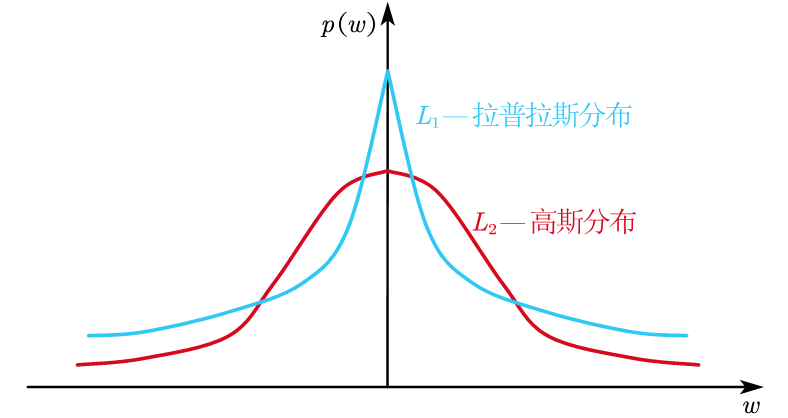
\includegraphics[width=\textwidth]{p_w.png}
	\caption{$L_1,L_2$先验概率分布}
	\label{fig:1}
\end{figure}

从图中可以看出$L_1$正则化的先验概率分布中,当$w$接近0的时候,$p\left( w \right)$更大,因此利用$L_1$正则化得到$w$的分量更可能为0,也就是说解更加稀疏,起到了特征选择的作用。而$L_2$正则化的先验概率分布更为平滑,相对更难得到为0的$w$分量,不过它也会让$w$的值趋近于0。
\subsubsection{梯度角度}

现在研究w的分量是否可以变为0,设$w=\left( w_1,w_2,...w_j \right) $
$$
\frac{\partial L_1\left( w \right)}{\partial w_j}=\frac{\partial \sum_{i=1}^N{\left( w^Tx_i-y_i \right) ^2}}{\partial w_j}+\frac{\partial \lambda \lVert w \rVert _1}{\partial w_j}
\\
=\sum_{i=1}^N{\left( w_{j}^{T}x_i-y_i \right) x_i+\lambda sign\left( w_j \right)}
$$
$$
\frac{\partial L_2\left( w \right)}{\partial w_j}=\frac{\partial \sum_{i=1}^N{\left( w^Tx_i-y_i \right) ^2}}{\partial w_j}+\frac{\partial \lambda \lVert w \rVert _{2}^{2}}{\partial w_j}
\\
=\sum_{i=1}^N{\left( w_{j}^{T}x_i-y_i \right) x_i+2\lambda w_j}
$$

可以看到,加入正则化后的导数可以看作是原本的线性回归损失函数的导数与正则项损失函数的导数的和。在导数=0时取极值,实际上就是分析导数为0这个点的原损失函数与正则项这两部分的导数大小的关系。

对于$L_1$正则化,只要保证正则项的系数大于原本的损失函数在0处的导数,那么$w_j=0$就是极值点,那么$w_j$就会收敛到0.

而对于$L_2$正则化,如果原本的损失函数在0处导数不为0,那么施加正则化项后在0处导数仍不为0,此时$w_j$不会为0。
因此,$L_1$更容易得到值为0的w分量(解变稀疏),也就是起到了特征选择作用。

\subsection{弹性网络}
弹性网络的损失函数为:
$$
L\left( w \right) =\sum_{i=1}^N{\left( y_i-w^Tx_i \right) ^2+r\lambda \lVert w \rVert _1+\frac{1-r}{2}\lambda \lVert w \rVert _{2}^{2}}
$$

可以看出,弹性网络将$L_1,L_2$结合,组成一个具有两种惩罚因素的单一模型:一个与L1范数成比例,另外一个与L2范数成比例。使用这种方式方法所得到的模型就像纯粹的Lasso回归一样稀疏,但同时具有与岭回归提供的一样的正则化能力。
\section{增加数据量/数据增强}
前面在VC角度解释过拟合时推导出了这个公式:

\noindent
有$1-\delta$的概率使:
$$
E_{out}\leqslant E_{in}+\sqrt{\frac{8}{N}\ln \left( \frac{4\left( 2N \right) ^{d_{vc}}}{\delta} \right)}
$$

可以看出$E_{in}$可以控制$E_{out}$的范围,而这取决于训练样本个数N和VC维数$d_{vc}$,训练样本越多,那么泛化误差$E_{out}$就可以越接近训练误差$E_{in}$。所以,我们可以考虑增加训练数据集的规模来防止过拟合。但训练数据有时难以获取,这是可以考虑使用数据增强来增加数据规模。
我们可以对数据集的每个数据做一些改动,比如对于图像,可以进行旋转、平移、翻转、裁剪、缩放等。这样就使得数据量变大了。
之前我看到过一个具体的应用例子:在KCF(核化相关滤波器)中,利用了循环矩阵来增加训练数据。这是一个目标跟踪算法,每一帧会利用当前跟踪框内的数据进行训练,该算法把框内的图像进行不断地平移来得到更多的训练样本,让模型的性能进一步提高了。
\section{提前停止训练}
很多学习算法都需要迭代来对模型的参数进行优化,迭代的越多意味着模型对训练集数据拟合的越好,为了防止过拟合,我们不希望模型把训练集数据拟合的过于好。迭代次数越多,训练误差越来越小,但泛化误差是先减小后增大,因此我们应该找到在验证集上误差最小的点,及时停止迭代。
%\clearpage
\begin{figure}[ht]
	\centering
	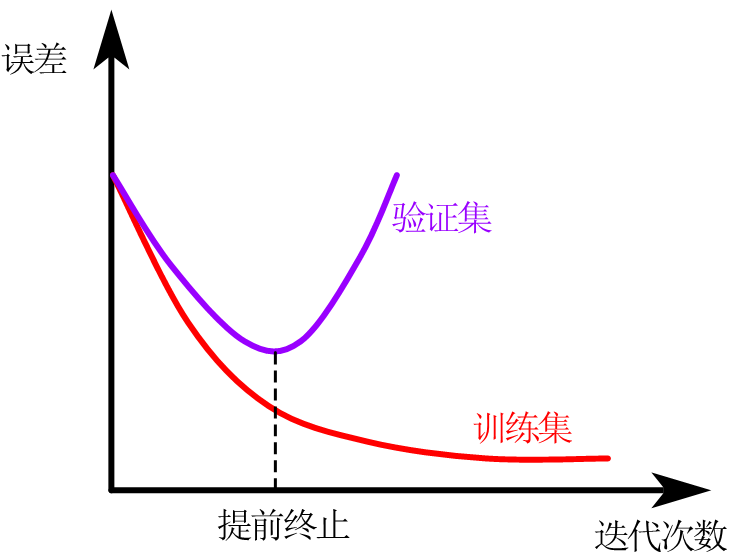
\includegraphics[width=\textwidth]{earlystop.png}
	\caption{误差与迭代次数的关系}
	\label{fig:1}
\end{figure}

\section{交叉验证——选择模型,衡量模型优劣}
交叉验证是一种可以较好的衡量模型优劣的方法。可以用于模型的选择(如在正则化中选择合适的正则项系数)。我们需要在假设集中选择出一个最好的假设作为我们最终学习到的函数,由前面的分析可知让训练误差最小并不是最优的,因此考虑将数据集中的一步分拆分出来作为测试集。比如可以把$70\%$的数据样本用于训练(训练集),剩余的$30\%$数据作为测试(验证集)。但这样相当于我们只使用了$70\%$的样本用来训练。因此应该寻找能使训练样本使用更充分的方法。
\subsection{k折交叉验证}
\paragraph*{k折交叉验证用于模型评估步骤}:

\noindent
1.将训练集$D$切分成 k 个不相交的子集,其中每一个子集的规模为 N/k 个训练样本。把这些子集称为 $D_1,...,D_k$。

\noindent
2.对 j = 1, ..., k,在$D_1\cup D_2\cup ...\cup D_{j-1}\cup D_{j+1}\cup ...\cup D_k$上(也就是除了$D_j$之外的其他所有子集)对模型进行训练,然后得到假设$g$。接下来把未被训练的$D_j$作为验证集对$g$进行测试,得到训练误差。对训练误差取平均值(也就是遍历所有的$j=1,...,k$后对每次结果计算然后取平均值),计算得到的值就当做是模型$g$的估计泛化误差,这个结果就是对模型性能的一个很好的评估。

通常这里进行折叠的次数k一般是10,即k=10。这样每次进行保留用于验证的数据块就只有 1/k ,这就比之前的 $30\%$ 要小多了,当然这样一来这个过程也要比最简单的交叉验证方法消耗更多算力成本,因为现在需要对每个模型都进行k次训练。

虽然通常选择都是设置 k=10,不过如果一些问题中数据量确实很匮乏,那有时候也可以走一点极端,设k=N,这样是为了每次能够尽可能多地利用数据,尽可能少地排除数据。这种情况下,我们需要在训练样本集D中除了某一个样本外的其他所有样本上进行训练,然后在保留出来的单独样本上进行检验。然后把计算出来的k=N个误差放到一起求平均值,这样就得到了对一个模型的泛化误差的估计。由于每次都保留了一个训练样本,所以这个方法就叫做弃一法交叉验证。

\paragraph*{k折交叉验证用于模型选择步骤}:

\noindent
1.将每个模型都用上述的模型评估步骤得到估计泛化误差,选择其中最小的那个作为最终的模型。

\noindent
2.用全部的数据集训练该模型,得到最终结果$g^*$。
\chapter{防止欠拟合的方法}
一般来讲,防止欠拟合比防止过拟合容易,因为防止欠拟合,只要让模型对训练数据集拟合好就可以了,这相对来讲容易做到,但防止过拟合比较困难,因为要让对训练集外的数据也有较小的误差,这些数据是未知的,因此更加困难。

通过前面的分析,防止欠拟合的基本思路就和防止过拟合的方法相反。如:增加模型的复杂度、选取或构造更多特征、增加训练集规模。
\chapter{编程实验——岭回归}
我主要编程实现了岭回归与线性回归(整体算法以及核心算法部分自己编写,sklearn只在数据预处理中使用),并比较性能。同时我也比较了不同正则化系数对结果带来的影响。全部实验结果与理论相符。

我生成了本次实验需要的数据集,包括训练集与测试集。并设计了理想的目标函数便于后面的观察对比,理想目标函数为$f\left( x \right) =-x^2+17x+3$,测试集选取了该函数曲线上的4个点,训练集选取了4个点,在该利用该函数得到函数值后加入了一些噪声,如图5.1所示。
\begin{figure}[ht]
	\centering
	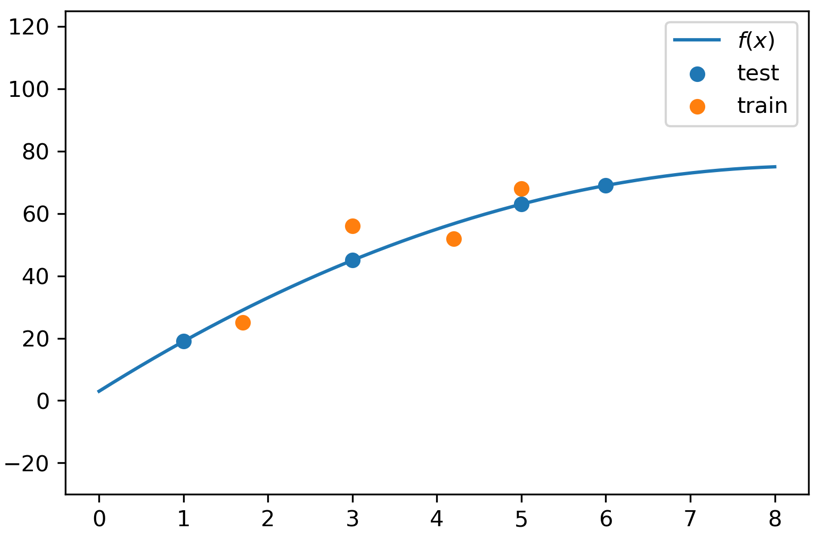
\includegraphics[width=\textwidth]{shujuji.png}
	\caption{实验数据集与理想目标函数}
	\label{fig:1}
\end{figure}

自己编写了线性回归以及岭回归算法。这里我利用的是多项式进行拟合。我设定最高次项为4,将训练集的样本特征映射到高维空间,映射函数为$\varPhi \left( x \right) =\left\{ 1,x,x^2,x^3,x^4 \right\}$。

然后,分别利用自己编写的线性回归、岭回归算法求得权值向量w,然后即得到结果曲线,如图5.2。
\begin{figure}[ht]
	\centering
	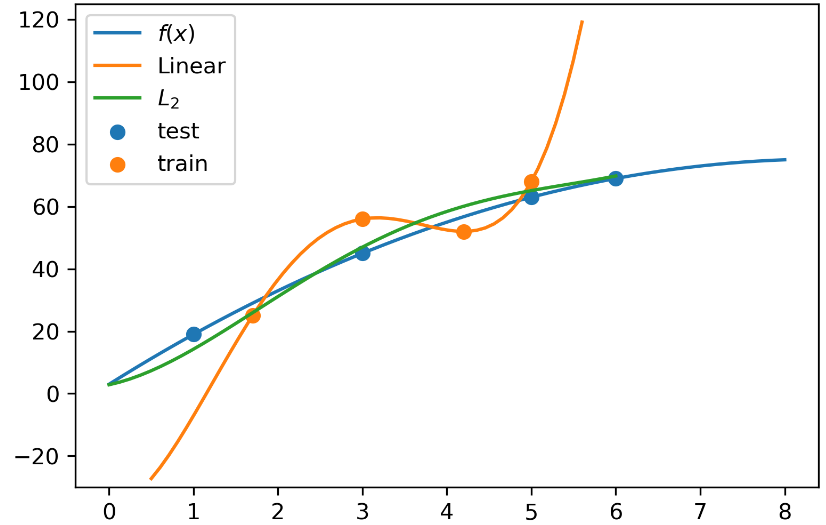
\includegraphics[width=\textwidth]{pltresult.png}
	\caption{线性回归、岭回归拟合结果}
	\label{fig:1}
\end{figure}

从图中可以看出,线性回归拟合的曲线完全拟合了训练集数据,即训练误差为0,但该曲线明显和目标函数f(x)有较大差距,这是因为训练集的样本过少,而模型的设定又偏复杂,因此产生了过拟合。与之相对,岭回归得到的拟合曲线虽然没有对训练集数据完全拟合,即训练误差不为0,但它的拟合曲线更接近理想的目标函数f(x)。

同时,我计算出了它们在测试集上的均方误差,也打印出了两条拟合曲线的各项系数,如图5.3。
\begin{figure}[ht]
	\centering
	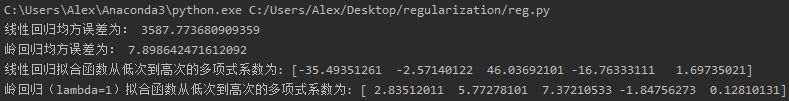
\includegraphics[width=\textwidth]{errresult.png}
	\caption{拟合曲线各项系数与在测试集上的均方误差}
	\label{fig:1}
\end{figure}

可以看出,岭回归得到拟合曲线的在测试集上的均方误差远小于线性回归,并且岭回归得到拟合曲线的各项系数得绝对值也小于线性回归的拟合曲线,这与理论相符。因为岭回归在线性回归的基础上加入了正则项,把权值w的大小加入了损失,尽量让w限制在靠近0的位置,这样也使得拟合曲线更加平滑,泛化性能更好,防止了过拟合。

然后,我探究了不同的正则项系数$\lambda$的取值对岭回归拟合曲线的影响,如图5.4、5.5。
\begin{figure}[ht]
	\centering
	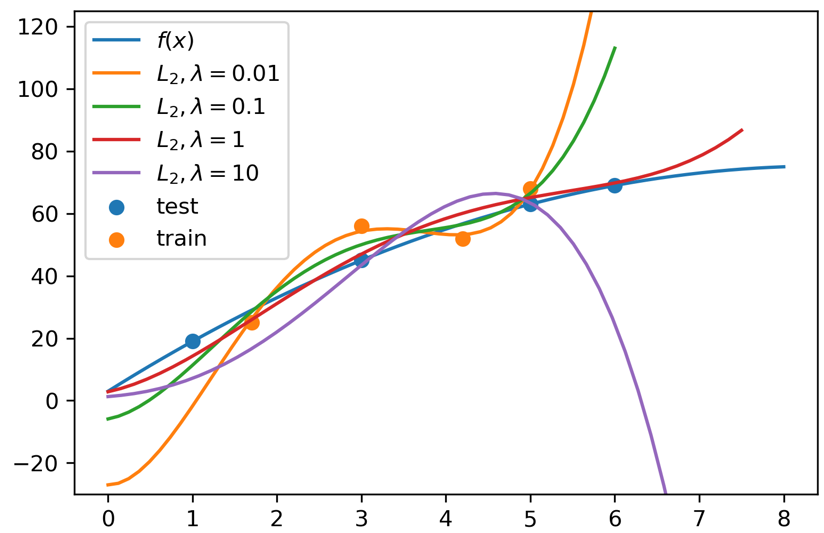
\includegraphics[width=\textwidth]{lambda.png}
	\caption{正则项系数$\lambda$对拟合曲线的影响}
	\label{fig:1}
\end{figure}
\begin{figure}[ht]
	\centering
	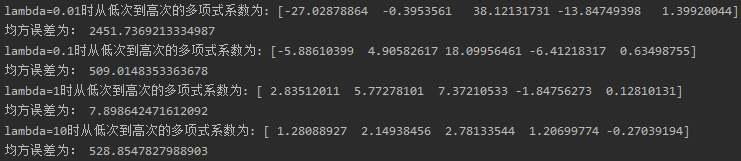
\includegraphics[width=\textwidth]{errresult1.png}
	\caption{正则项系数$\lambda$对拟合曲线各项系数和均方误差的影响}
	\label{fig:1}
\end{figure}

可以看出,$\lambda$越小,越接近线性回归,$\lambda$越大,越平滑,w各分量越小。在性能上并不是说$\lambda$越大越好,如$\lambda=10$时的拟合曲线也与目标函数f(x)差很远。在一般情况下可以借助交叉验证,选择合适的$\lambda$。
\chapter{总结}
欠拟合与过拟合是机器学习的基本问题。一般来讲解决欠拟合比解决过拟合容易。通过两个角度进行理论推导说明了模型复杂度、样本个数会影响模型的表现,因此避免过拟合和欠拟合主要需要权衡模型复杂度,复杂度过低容易欠拟合,过高容易过拟合,而样本数则越多越好。正则化是一种改善过拟合的方法,目的是让模型复杂度降低,通过让权值接近0来实现,使得曲线更加平缓,增强泛化性能,而$L_1,L_2$正则化在效果上有一些区别,这可以通过原理来解释。数据增强的目的是增加样本数量,提前停止训练是为了不让模型拟合的过好而降低泛化性能,交叉验证是一种很好的衡量模型性能的方法,也可以用来进行模型的选择。
%此处结束正文-------------------------------------------------------------------------------------------------
%%%============================================================================================================%%%

%%%=== 参考文献 ========%%%
\cleardoublepage\phantomsection
\addcontentsline{toc}{chapter}{参考文献}
\renewcommand{\baselinestretch}{1.6}
\begin{thebibliography}{00}

  \bibitem{r1} 林轩田. 《机器学习基石》. \url{https://www.bilibili.com/video/BV1Cx411i7op?p=26}
  
  \bibitem{r2} Andrew Ng. 《CS229:Machine Learning》. \url{https://www.bilibili.com/video/BV1xb411M7sn}
  
  \bibitem{r3} 周志华. 《机器学习》 [M]. 北京:清华大学出版社,2012:155-170.

  \bibitem{r3} shuhuai008. 机器学习白板推导系列. \url{https://space.bilibili.com/97068901/}.
  
  \bibitem{r4} Microstrong. 偏差(Bias)与方差(Variance). \url{https://zhuanlan.zhihu.com/p/38853908}.
  
  \bibitem{r4} ser jamie. l1 相比于 l2 为什么容易获得稀疏解?. \url{https://www.zhihu.com/question/37096933/answer/475278057}.
  

\end{thebibliography}

\cleardoublepage
\end{document}





